\documentclass{article}
\usepackage[utf8]{inputenc}
\usepackage[english]{babel}
\usepackage{graphicx}
\usepackage{hyperref}
\usepackage{array}
\hypersetup{
    colorlinks=true,
    linkcolor=blue,
    filecolor=magenta,      
    urlcolor=cyan,
    pdftitle={Overleaf Example},
    pdfpagemode=FullScreen,
    }
%Path relative to the .tex file containing the \includegraphics command
\graphicspath{ {./images/} }
\pagestyle{fancy}
\fancyhf{}
\rhead{}


%paragraph indentation
\setlength{\parindent}{4em} 

%paragraph spacing
\setlength{\parskip}{1em}

%Line spacing
\renewcommand{\baselinestretch}{1.5}

\usepackage{blindtext}


\begin{document}

\addcontentsline{toc}{section}{Unnumbered Section}
\begin{center}
 \section*{Introduction to Linux and Shell Script}  
\end{center}


\addcontentsline{toc}{section}{Unnumbered Section}
\begin{center}
 \section*{Introduction to Linux}  
\end{center}


\addcontentsline{toc}{section}{Unnumbered Section}
\section*{What is an Operating System (or operating system in a computer)?}

\noindent
Operating System (OS) is a software that manages a computer's resources, especially the allocation of those resources among other programs. Typical resources include the central processing unit (CPU), computer memory, file storage, input/output (I/O) devices, and network connections.\\
Operating System is system software. The communication between a user and a system takes place with the help of an operating systems. Windows, Linux, and Android are examples of operating systems that enable the user to use programs like MS Office, Notepad, and games on the computer or mobile phone.
\\
\addcontentsline{toc}{section}{Unnumbered Section}
\section*{List the major Operating Systems.}
\noindent
For computers : Unix, Linux, Wondos, Apple macOS (Macintosh Operating System)
For mobile Phones/Tabs : Android, iOS
\addcontentsline{toc}{section}{Unnumbered Section}
\section*{Linux as an Operating System}

\noindent
Linux is a family of open-source Unix-like operating systems based on the Linux kernel, an operating system kernel first released on September 17, 1991, by Linus Torvalds. Linux is typically packaged in a Linux distribution.\\
Popular Linux distributions include Debian, Fedora Linux, and Ubuntu, which in itself has many different distributions and modifications, Including Lubuntu and Xubuntu. Commercial distributions include Red Hat Enterprise Linux and SUSE Linux Enterprise. Desktop Linux distributions include a windowing system such as X11 or Wayland, and a desktop environment such as GNOME or KDE Plasma. Distributions intended for servers may omit graphics altogether, or include a solution stack such as LAMP. Because Linux is freely redistributable, anyone may create a distribution for any purpose.
Linux was originally developed for personal computers based on the Intel x86 architecture, but has since been ported to more platforms than any other operating system.\\
Linux also runs on embedded systems, i.e. devices whose operating system is typically built into the firmware and is highly tailored to the system. This includes routers, automation controls, smart home technology, televisions (Samsung and LG Smart TVs use Tizen and WebOS, respectively), automobiles (for example, Tesla, Audi, Mercedes-Benz, Hyundai, and Toyota all rely on Linux), digital video recorders, video game consoles, and smartwatches. The Falcon 9's and the Dragon 2's avionics use a customized version of Linux.\\
Linux is one of the most prominent examples of free and open-source software collaboration. The source code may be used, modified and distributed commercially or non-commercially by anyone under the terms of its respective licenses, such as the GNU General Public License.

\addcontentsline{toc}{section}{Unnumbered Section}
\section*{Creation}
\noindent
In 1991, while attending the University of Helsinki, Torvalds became curious about operating systems. Frustrated by the licensing of MINIX, which at the time limited it to educational use only, he began to work on his own operating system kernel, which eventually became the Linux kernel.\\
Torvalds began the development of the Linux kernel on MINIX and applications written for MINIX were also used on Linux. Later, Linux matured and further Linux kernel development took place on Linux systems. GNU applications also replaced all MINIX components, because it was advantageous to use the freely available code from the GNU Project with the fledgling operating system; code licensed under the GNU GPL can be reused in other computer programs as long as they also are released under the same or a compatible license. Torvalds initiated a switch from his original license, which prohibited commercial redistribution, to the GNU GPL. Developers worked to integrate GNU components with the Linux kernel, making a fully functional and free operating system.

\begin{center}
    \resizebox{0.7\textwidth}{!}{
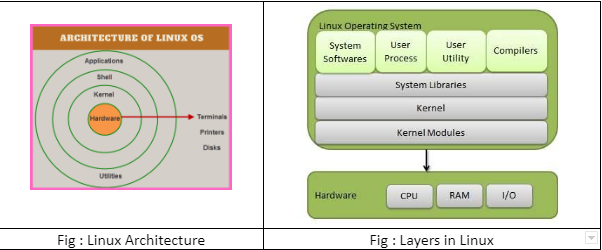
\includegraphics{Linux_layers_and_architecture.png}
}
\end{center}

\addcontentsline{toc}{section}{Unnumbered Section}
\section*{User interface}
\noindent
The user interface, also known as the shell, is either a command-line interface (CLI), a graphical user interface (GUI), or controls attached to the associated hardware, which is common for embedded systems. For desktop systems, the default user interface is usually graphical, although the CLI is commonly available through terminal emulator windows or on a separate virtual console.\\

CLI shells are text-based user interfaces, which use text for both input and output. The dominant shell used in Linux is the Bourne-Again Shell (bash), originally developed for the GNU project. Most low-level Linux components, including various parts of the userland, use the CLI exclusively. The CLI is particularly suited for automation of repetitive or delayed tasks and provides very simple inter-process communication.\\

On desktop systems, the most popular user interfaces are the GUI shells, packaged together with extensive desktop environments, such as KDE Plasma, GNOME, MATE, Cinnamon, LXDE, Pantheon and Xfce, though a variety of additional user interfaces exist. Most popular user interfaces are based on the X Window System, often simply called "X". It provides network transparency and permits a graphical application running on one system to be displayed on another where a user may interact with the application; however, certain extensions of the X Window System are not capable of working over the network. Several X display servers exist, with the reference implementation, X.Org Server, being the most popular.\\
Server distributions might provide a command-line interface for developers and administrators, but provide a custom interface towards end-users, designed for the use-case of the system. This custom interface is accessed through a client that resides on another system, not necessarily Linux based.\\

\addcontentsline{toc}{section}{Unnumbered Section}
\begin{center}
    \section*{Linux Commands}
\end{center}
\noindent
Linux commands are handy to operate Linux and Unix Systems and also to handle Cloud Computing. \\

\addcontentsline{toc}{section}{Unnumbered Section}
\textcolor{blue}{System Monitoring}\\
\noindent
\# Display Linux system information\\
uname -a\\
\# Display kernel release information\\
uname -r\\
\# Show which version of Red Hat installed\\
cat /etc/redhat-release\\
\# Show how long the system has been running + load\\
uptime\\
\# Show system host name\\
hostname\\
\# Display all local IP addresses of the host.\\
hostname -I\\
\# Show system reboot history\\
last reboot\\
\# Show the current date and time\\
date\\
\# Show this month's calendar\\
cal\\
\# Display who is online\\
w\\
\# Who you are logged in as\\
whoami\\

\addcontentsline{toc}{section}{Unnumbered Section}
\textcolor{blue}{Hardware Information}\\
\noindent
\# Display messages in kernel ring buffer\\
dmesg\\
\# Display CPU information\\
cat /proc/cpuinfo\\
\# Display memory information\\
cat /proc/meminfo\\
\# Display free and used memory ( -h for human readable, -m for MB, -g for GB.)\\
free -h\\
\# Display PCI devices\\
lspci -tv\\
\# Display USB devices\\
lsusb -tv\\
\# Display DMI/SMBIOS (hardware info) from the BIOS\\
dmidecode\\
\# Show info about disk sda\\
hdparm -i /dev/sda\\
\# Perform a read speed test on disk sda\\
hdparm -tT /dev/sda\\
\# Test for unreadable blocks on disk sda\\
badblocks -s /dev/sda\\

\addcontentsline{toc}{section}{Unnumbered Section}
\textcolor{blue}{Performance Monitoring and Statistics}\\
\noindent
\# Display and manage the top processes\\
top\\
\# Interactive process viewer (top alternative)\\
htop\\
\# Display processor related statistics\\
mpstat 1\\
\# Display virtual memory statistics\\
vmstat 1\\
\# Display I/O statistics\\
iostat 1\\
\# Display the last 100 syslog messages  (Use /var/log/syslog for Debian based systems.)\\
tail -100 /var/log/messages\\
\# Capture and display all packets on interface eth0\\
tcpdump -i eth0\\
\# Monitor all traffic on port 80 ( HTTP )\\
tcpdump -i eth0 'port 80'\\
\# List all open files on the system\\
lsof\\
\# List files opened by user\\
lsof -u user\\
\# Display free and used memory ( -h for human readable, -m for MB, -g for GB.)\\
free -h\\
\# Execute "df -h", showing periodic updates\\
watch df –h\\

\addcontentsline{toc}{section}{Unnumbered Section}
\textcolor{blue}{User information and management }\\
\noindent
\# Display the user and group ids of your current user.\\
id\\
\# Display the last users who have logged onto the system.\\
last\\
\# Show who is logged into the system.\\
who\\
\# Show who is logged in and what they are doing.\\
w\\
\# Create a group named "test".\\
groupadd test\\
\# Create an account named john, with a comment of "John Smith" and create the user's home directory.\\
useradd -c "John Smith" -m john\\
\# Delete the john account.\\
userdel john\\
\# Add the john account to the sales group\\
usermod -aG sales john\\

\addcontentsline{toc}{section}{Unnumbered Section}
\textcolor{blue}{File and Directory Commands }\\
\noindent
\# List all files in a long listing (detailed) format\\
ls -al\\
\# Display the present working directory\\
pwd\\
\# Create a directory\\
mkdir directory\\
\# Remove (delete) file\\
rm file\\
\# Remove the directory and its contents recursively\\
rm -r directory\\
\# Force removal of file without prompting for confirmation\\
rm -f file\\
\# Forcefully remove directory recursively\\
rm -rf directory
\# Copy file1 to file2\\
cp file1 file2\\
\# Copy source\_directory recursively to destination. If destination exists, copy source\_directory into destination, otherwise create destination with the contents of source\_directory.\\
cp -r source\_directory destination\\
\# Rename or move file1 to file2. If file2 is an existing directory, move file1 into directory file2\\
mv file1 file2\\
\# Create symbolic link to linkname\\
ln -s /path/to/file linkname\\
\# Create an empty file or update the access and modification times of file.\\
touch file\\
\# View the contents of file\\
cat file\\
\# Browse through a text file\\
less file\\
\# Display the first 10 lines of file\\
head file\\
\# Display the last 10 lines of file\\
tail file\\
\# Display the last 10 lines of file and "follow" the file as it grows.\\
tail -f file\\

\addcontentsline{toc}{section}{Unnumbered Section}
\textcolor{blue}{Process management }\\
\noindent
\# Display your currently running processes\\
ps\\
\# Display all the currently running processes on the system.\\
ps -ef\\
\# Display process information for processname\\
ps -ef | grep processname\\
\# Display and manage the top processes\\
top\\
\# Interactive process viewer (top alternative)\\
htop\\
\# Kill process with process ID of pid\\
kill pid\\
\# Kill all processes named processname\\
killall processname\\
\# Start program in the background\\
program &\\
\# Display stopped or background jobs\\
bg\\
\# Brings the most recent background job to foreground\\
fg\\
\# Brings job n to the foreground\\
fg n\\

\addcontentsline{toc}{section}{Unnumbered Section}
\textcolor{blue}{File Permissions  }\\
\noindent
\begin{center}
    \resizebox{0.7\textwidth}{!}{
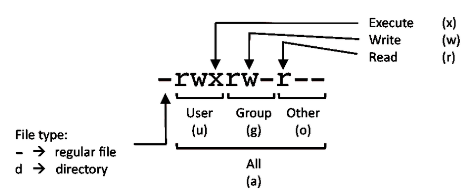
\includegraphics{file_permission.png}
}
\end{center}
PERMISSION      EXAMPLE\\
U   G   W\\
        rwx rwx rwx     chmod 777 filename\\
        rwx rwx r-x     chmod 775 filename\\
        rwx r-x r-x     chmod 755 filename\\
        rw- rw- r--     chmod 664 filename\\
        rw- r-- r--     chmod 644 filename\\
\# NOTE: Use 777 sparingly!\\
LEGEND\\
U = User\\
G = Group\\
W = World\\
r = Read\\
w = write\\
x = execute\\
- = no access\\

\addcontentsline{toc}{section}{Unnumbered Section}
\textcolor{blue}{Installing Packages }\\
\noindent
\# Search for a package by keyword.\\
yum search keyword\\
\# Install package.\\
yum install package\\
\# Display description and summary information about package.\\
yum info package\\
\# Install package from local file named package.rpm\\
rpm -i package.rpm\\
\# Remove/uninstall package.\\
yum remove package\\
\# Install software from source code.\\
tar zxvf sourcecode.tar.gz\\
cd sourcecode\\
./configure\\
make\\
make install\\

\addcontentsline{toc}{section}{Unnumbered Section}
\textcolor{blue}{Search Commands}\\
\noindent
\# Search for pattern in file\\
grep pattern file\\
\# Search recursively for pattern in directory\\
grep -r pattern directory\\
\# Find files and directories by name\\
locate name\\
\# Find files in /home/john that start with "prefix".\\
find /home/john -name 'prefix*'\\
\# Find files larger than 100MB in /home\\
find /home -size +100M\\

\addcontentsline{toc}{section}{Unnumbered Section}
\textcolor{blue}{SSH Logins}\\
\noindent
\# Connect to host as your local username.\\
ssh host\\
\# Connect to host as user\\
ssh user@host\\
\# Connect to host using port\\
ssh -p port user@host\\

\addcontentsline{toc}{section}{Unnumbered Section}
\textcolor{blue}{File Transfers}\\
\noindent
\# Secure copy file.txt to the /tmp folder on server\\
scp file.txt server:/tmp\\
\# Copy *.html files from server to the local /tmp folder.\\
scp server:/var/www/*.html /tmp\\
\# Copy all files and directories recursively from server to the current system's /tmp folder.\\
scp -r server:/var/www /tmp\\
\# Synchronize /home to /backups/home\\
rsync -a /home /backups/\\
\# Synchronize files/directories between the local and remote system with compression enabled\\
rsync -avz /home server:/backups/\\

\addcontentsline{toc}{section}{Unnumbered Section}
\textcolor{blue}{Directory Navigation}\\
\noindent
\# To go up one level of the directory tree.  (Change into the parent directory.)\\
cd ..
\# Go to the \$HOME directory\\
cd\\
\# Change to the /etc directory\\
cd /etc\\

\addcontentsline{toc}{section}{Unnumbered Section}
\begin{center}
    \textcolor{red}{Shell Scripting}\\
\end{center}

\textcolor{blue}{Linux Text Processing with Vim}\\
Vim is a text editor I can identify with: Vim and I are both 90's babies, and we prefer to work smarter, not harder. There are a multitude of reasons to learn Vim, from its simple navigation tools to its quick and dirty character correction.\\
What is Vim?\\
The name Vim is an acronym for Vi Improved. This editor is an enhanced version of the Vi text editor that we all know and love, and is normally seen in a CLI form; however, it does have a GUI version available for standard desktop use. Vim allows you to merge files using vimdiff—which is not the same as diff, the comparison utility—as well as an autocomplete feature and a comparison mode that is similar to the diff utility. This editor's real change and utility is supporting plugins and multiple scripting languages such as Perl and Python. Also included is support for compression functions such as tar and zip, as well as network transfer protocols such as SSH, FTP, and HTTP.\\ 

\addcontentsline{toc}{section}{Unnumbered Section}
\section*{Vim's common modes}
The Vim editor has three modes that determine how the editor functions: Normal (or Command), Insert, and GUI.\\

\addcontentsline{toc}{section}{Unnumbered Section}
\section*{Normal mode}
Normal mode allows you to give commands to the editor. Functions such as the following can be found here:\\
    :w to write/save.\\
    :q to quit.\\
    :w <filename.txt> to name a new file.\\
    :q! to quit without saving the changes to the file\\
Press the Esc key to start the Normal mode and enter :(desired command) [Enter] to perform your intended task. For example, if I was working in a new file and wanted to name it 'file.txt', I would use the following:\\ 
:w file.txt [ENTER]\\

\addcontentsline{toc}{section}{Unnumbered Section}
\section*{Insert mode}
If you have made it this far, you probably know what the Insert mode does. However, for those who don't, if you press the I key (lowercase i) once you will see the "INSERT" prompt at the bottom of the screen, indicating that you can now edit or add text.\\
To exit this mode and return to Normal mode, press the Esc key once.\\ 

\addcontentsline{toc}{section}{Unnumbered Section}
\section*{Insert mode}
GUI mode is only available in some environments. It offers a graphical, point-and-click interface to be utilized with a mouse and keyboard.\\

\addcontentsline{toc}{section}{Unnumbered Section}
\section*{Vim tips and tricks}
Now, imagine Vim being that shady guy on the corner in a trenchcoat selling faux Rolex watches from inside his lapel, only instead of knockoff watches, VIM has tricks and shortcuts on offer. Seriously, there are too many to list in this article, but I will list some of my favorites here:\\ 
    dd removes all text from the current line (deleting the full line) and saves the removed text to the clipboard.\\ 
    p pastes (puts) anything from the Vim clipboard to the current cursor, and pairs nicely with the full line delete shortcut above.\\ 
    r replaces a character and is great for a quick correction.\\

\addcontentsline{toc}{section}{Unnumbered Section}
\section*{Using r is a bit more complicated than the others:}
\begin{itemize}
    \item Press Esc to enter Normal mode.
   \item  Move the cursor onto the character you wish to correct.
   \item  Type r followed by the character that you wish to use.
\end{itemize}
For example, "Goodbee" can be edited to "Goodbye" by highlighting the first "e" and then entering ry.

\addcontentsline{toc}{section}{Unnumbered Section}
\textcolor{blue}{Shell Scripts:}\\
\noindent
A shell script is a computer program designed to be run by the Unix/Linux shell which could be one of the following:\\
\begin{itemize}
    \item The Bourne Shell
    \item The C Shell
    \item The Korn Shell
    \item The GNU Bourne-Again Shell
\end{itemize}
A \textbf{shell is a command-line interpreter} and typical operations performed by shell scripts include file manipulation, program execution, and printing text.

\addcontentsline{toc}{section}{Unnumbered Section}
\section*{Extended Shell Scripts}
Shell scripts have several required constructs that tell the shell environment what to do and when to do it. Of course, most scripts are more complex than the above one.\\
The shell is, after all, a real programming language, complete with variables, control structures, and so forth. No matter how complicated a script gets, it is still just a list of commands executed sequentially.\\
The following script uses the read command which takes the input from the keyboard and assigns it as the value of the variable PERSON and finally prints it on STDOUT.\\
\#!/bin/sh\\
\# Author : Siddhartha\\
\# Copyright (c) TalentSprint.com\\
\# Script follows here:\\
echo "What is your name?"\\
read PERSON\\
echo "Hello, \$PERSON"\\

\addcontentsline{toc}{section}{Unnumbered Section}
\section*{Here is a sample run of the script −}
\$./test.sh\\
What is your name?\\
Siddhartha\\
Hello, Siddhartha\\
\$

\addcontentsline{toc}{section}{Unnumbered Section}
\section*{Shell Scripts}
The basic concept of a shell script is a list of commands, which are listed in the order of execution. A good shell script will have comments, preceded by # sign, describing the steps.\\
There are conditional tests, such as value A is greater than value B, loops allowing us to go through massive amounts of data, files to read and store data, and variables to read and store data, and the script may include functions.\\
We are going to write many scripts in the next sections. It would be a simple text file in which we would put all our commands and several other required constructs that tell the shell environment what to do and when to do it.\\
Shell scripts and functions are both interpreted. This means they are not compiled.
A variable is a character string to which we assign a value. The value assigned could be a number, text, filename, device, or any other type of data.\\
A variable is nothing more than a pointer to the actual data. The shell enables you to create, assign, and delete variables.\\

\addcontentsline{toc}{section}{Unnumbered Section}
\section*{Variable Names}
The name of a variable can contain only letters (a to z or A to Z), numbers ( 0 to 9) or the underscore character ( \_).\\
By convention, Unix shell variables will have their names in UPPERCASE.\\
The following examples are valid variable names −\\
\_ALI\\
TOKEN\_A\\
VAR\_1\\
VAR\_2\\
Following are the examples of invalid variable names −\\
2\_VAR\\
-VARIABLE\\
VAR1-VAR2\\
VAR\_A!\\
The reason you cannot use other characters such as !, *, or - is that these characters have a special meaning for the shell.\\

\addcontentsline{toc}{section}{Unnumbered Section}
\section*{Defining Variables}
Variables are defined as follows −\\
variable\_name=variable\_value\\
For example −\\
NAME="Siddhartha G"\\
The above example defines the variable NAME and assigns the value "Siddhartha G" to it. Variables of this type are called scalar variables. A scalar variable can hold only one value at a time.\\
Shell enables you to store any value you want in a variable. For example −\\
VAR1="Siddhartha G"\\
VAR2=100\\
Accessing Values\\
To access the value stored in a variable, prefix its name with the dollar sign (\$) −\\
For example, the following script will access the value of defined variable NAME and print it on STDOUT −\\
\#!/bin/sh\\
NAME="Siddhartha G"\\
echo \$NAME\\
The above script will produce the following value −\\
Siddhartha G\\

\addcontentsline{toc}{section}{Unnumbered Section}
\section*{Read-only Variables}
Shell provides a way to mark variables as read-only by using the read-only command. After a variable is marked read-only, its value cannot be changed.\\
For example, the following script generates an error while trying to change the value of NAME −\\
\#!/bin/sh\\
NAME="Siddhartha G"\\
readonly NAME\\
NAME="TalentSprint"\\
The above script will generate the following result −\\
/bin/sh: NAME: This variable is read only.\\

\addcontentsline{toc}{section}{Unnumbered Section}
\section*{Unsetting Variables}
Unsetting or deleting a variable directs the shell to remove the variable from the list of variables that it tracks. Once you unset a variable, you cannot access the stored value in the variable.\\
Following is the syntax to unset a defined variable using the unset command −\\
unset variable\_name\\
The above command unsets the value of a defined variable. Here is a simple example that demonstrates how the command works −\\
\#!/bin/sh\\
NAME="Siddhartha G"\\
unset NAME\\
echo \$NAME\\
The above example does not print anything. You cannot use the unset command to unset variables that are marked read only.\\

\addcontentsline{toc}{section}{Unnumbered Section}
\section*{Variable Types}
When a shell is running, three main types of variables are present −\\
    Local Variables : A local variable is a variable that is present within the current instance of the shell. It is not available to programs that are started by the shell. They are set at the command prompt.\\
    Environment Variables : An environment variable is available to any child process of the shell. Some programs need environment variables in order to function correctly. Usually, a shell script defines only those environment variables that are needed by the programs that it runs.\\
    Shell Variables : A shell variable is a special variable that is set by the shell and is required by the shell in order to function correctly. Some of these variables are environment variables whereas others are local variables.\\
Now we will discuss in detail about special variable in Unix. In one of our previous topic, we understood how to be careful when we use certain non alphanumeric characters in variable names. This is because those characters are used in the names of special Unix variables. These variables are reserved for specific functions.\\
For example, the \$ character represents the process ID number, or PID, of the current shell −\\
\$echo \$\$\\
The above command writes the PID of the current shell :\\
29949\\
The following table shows a number of special variables that you can use in your shell scripts :\\
\noindent
\begin{itemize}
    \item \$0:The filename of the current script.
    \item \$n":These variables correspond to the arguments with which a script was invoked. Here n is a positive decimal number corresponding to the position of an argument (the first argument is \$1, the second argument is \$2, and so on).
    \item \$\#:The number of arguments supplied to a script.\\
    \item \$*:All the arguments are double quoted. If a script receives two arguments, \$* is equivalent to \$1 \$2.\\
    \item \$@: All the arguments are individually double quoted. If a script receives two arguments, \$@ is equivalent to \$1 \$2.\\
    \item \$?:The exit status of the last command executed.\\
    \item \$\$:The process number of the current shell. For shell scripts, this is the process ID under which they are executing.\\
    \item \$!
\end{itemize}

\addcontentsline{toc}{section}{Unnumbered Section}
\section*{Command-Line Arguments}
The command-line arguments \$1, \$2, \$3, ...\$9 are positional parameters, with \$0 pointing to the actual command, program, shell script, or function and \$1, \$2, \$3, ...\$9 as the arguments to the command.\\
Following script uses various special variables related to the command line :\\
\#!/bin/sh\\
echo "File Name: \$0"\\
echo "First Parameter : \$1"\\
echo "Second Parameter : \$2"\\
echo "Quoted Values: \$@"\\
echo "Quoted Values: \$*"\\
echo "Total Number of Parameters : \$#"\\
Here is a sample run for the above script :\\
\$./test.sh Siddhartha G\\
File Name : ./test.sh\\
First Parameter : Siddhartha\\
Second Parameter : G\\
Quoted Values: Siddhartha G\\
Quoted Values: Siddhartha G\\
Total Number of Parameters : 2\\

\addcontentsline{toc}{section}{Unnumbered Section}
\section*{Special Parameters \$* and \$@}
There are special parameters that allow accessing all the command-line arguments at once. \$* and \$@ both will act the same unless they are enclosed in double quotes, "".\\
Both the parameters specify the command-line arguments. However, the "\$*" special parameter takes the entire list as one argument with spaces between and the "\$@" special parameter takes the entire list and separates it into separate arguments.
We can write the shell script as shown below to process an unknown number of command line arguments with either the $* or $@ special parameters :\\
\#!/bin/sh\\
for TOKEN in \$*\\
do\\
   echo \$TOKEN\\
done\\
Here is a sample run for the above script :\\
\$./test.sh Siddhartha G Hyderabad Telangana India\\
Siddhartha\\
G\\
Hyderabad\\
Telangana\\
India\\
Note : Here do...done is a kind of loop that will be covered in a subsequent tutorial.\\
Exit Status\\
The \$? variable represents the exit status of the previous command.\\
Exit status is a numerical value returned by every command upon its completion. As a rule, most commands return an exit status of 0 if they were successful, and 1 if they were unsuccessful.\\
Some commands return additional exit statuses for particular reasons. For example, some commands differentiate between kinds of errors and will return various exit values depending on the specific type of failure.\\
Following is the example of successful command :
\$./test.sh Siddhartha G\\
File Name : ./test.sh\\
First Parameter : Siddhartha\\
Second Parameter : G\\
Quoted Values: Siddhartha G\\
Quoted Values: Siddhartha G\\
Total Number of Parameters : 2\\
\$echo \$?\\
0\\
\$\\
Now we will discuss how to use shell arrays in Unix. A shell variable is capable enough to hold a single value. These variables are called scalar variables.\\
Shell supports a different type of variable called an array variable. This can hold multiple values at the same time. Arrays provide a method of grouping a set of variables. Instead of creating a new name for each variable that is required, you can use a single array variable that stores all the other variables.\\
All the naming rules discussed for Shell Variables would be applicable while naming arrays.\\
Defining Array Values\\
The difference between an array variable and a scalar variable can be explained as follows.\\
Suppose you are trying to represent the names of various students as a set of variables. Each of the individual variables is a scalar variable as follows :\\
NAME01="World"\\
NAME02="Asia"\\
NAME03="India"\\
NAME04="Telangana"\\
NAME05="India"\\
We can use a single array to store all the above mentioned names. Following is the simplest method of creating an array variable. This helps assign a value to one of its indices.\\
array\_name[index]=value\\
Here array\_name is the name of the array, index is the index of the item in the array that you want to set, and value is the value you want to set for that item.
As an example, the following commands :\\
NAME[0]="World"\\
NAME[1]="Asia"\\
NAME[2]="India"\\
NAME[3]="Telangana"\\
NAME[4]="Hyderabad"\\
If you are using the ksh shell, here is the syntax of array initialization :\\
set -A array\_name value1 value2 ... valuen\\
If you are using the bash shell, here is the syntax of array initialization :\\
array\_name=(value1 ... valuen)\\
Accessing Array Values\\
After you have set any array variable, you access it as follows :\\
\$\{array\_name[index]\}\\
Here array\_name is the name of the array, and index is the index of the value to be accessed. Following is an example to understand the concept :\\
\#!/bin/sh\\
NAME[0]="World"\\
NAME[1]="Asia"\\
NAME[2]="India"
NAME[3]="Telangana"\\
NAME[4]="Hyderabad"\\
echo "First Index: \${NAME[0]}"\\
echo "Second Index: \${NAME[1]}"\\
The above example will generate the following result :\\
\$./test.sh\\
First Index: World\\
Second Index: Asia\\
You can access all the items in an array in one of the following ways :\\
\$\{array\_name[*]\}\\
\$\{array\_name[@]\}\\
Here array\_name is the name of the array you are interested in. Following example will help you understand the concept :\\
\#!/bin/sh\\
NAME[0]="Asia"\\
NAME[1]="Asia"\\
NAME[2]="India"\\
NAME[3]="Telangana"\\
NAME[4]="Hyderabad"\\
echo "First Method: \$\{NAME[*]\}"\\
echo "Second Method: \$\{NAME[@]\}"\\
The above example will generate the following result :\\
\$./test.sh\\
First Method: World Asia India Telangana Hyderabad\\
Second Method: World Asia India Telangana Hyderabad\\

\addcontentsline{toc}{section}{Unnumbered Section}
\section*{Operators }
There are various operators supported by each shell. We will discuss in detail about Bourne shell (default shell) in this chapter.\\
We will now discuss the following operators :\\
\begin{itemize}
    \item Arithmetic Operators
    \item Relational Operators
    \item Boolean Operators
    \item String Operators
    \item File Test Operators
\end{itemize}
Bourne shell didn't originally have any mechanism to perform simple arithmetic operations but it uses external programs, either awk or expr.\\
The following example shows how to add two numbers :\\
\#!/bin/sh\\
val=`expr 2 + 2`\\
echo "Total value : \$val"\\
The above script will generate the following result :\\
Total value : 4\\
The following points need to be considered while adding :\\
    There must be spaces between operators and expressions. For example, 2+2 is not correct; it should be written as 2 + 2.\\
    The complete expression should be enclosed between ‘ ‘, called the backtick.\\

\addcontentsline{toc}{section}{Unnumbered Section}
\section*{Arithmetic Operators}
The following arithmetic operators are supported by Bourne Shell.\\
Assume variable a holds 10 and variable b holds 20 then :
\begin{center}
    \resizebox{0.7\textwidth}{!}{
\includegraphics{Arthematic_operators.png}
}
\end{center}
It is very important to understand that all the conditional expressions should be inside square braces with spaces around them, for example [ \$a == \$b ] is correct whereas, [\$a==\$b] is incorrect.\\
All the arithmetical calculations are done using long integers.

\addcontentsline{toc}{section}{Unnumbered Section}
\section*{Relational Operators}
Bourne Shell supports the following relational operators that are specific to numeric values. These operators do not work for string values unless their value is numeric.\\
For example, following operators will work to check a relation between 10 and 20 as well as in between "10" and "20" but not in between "ten" and "twenty".\\
Assume variable a holds 10 and variable b holds 20 then :\\
\begin{center}
    \resizebox{0.7\textwidth}{!}{
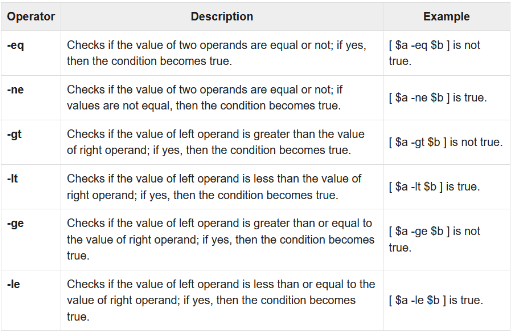
\includegraphics{Relational_operators.png}
}
\end{center}
It is very important to understand that all the conditional expressions should be placed inside square braces with spaces around them. For example, [ \$a $<$= \$b ] is correct whereas, [\$a $<$= \$b] is incorrect.\\

\addcontentsline{toc}{section}{Unnumbered Section}
\section*{Boolean Operators}
The following Boolean operators are supported by the Bourne Shell.\\
Assume variable a holds 10 and variable b holds 20 then :\\
\begin{center}
    \resizebox{0.7\textwidth}{!}{
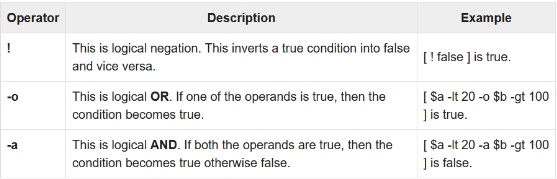
\includegraphics{Boolean_Operator.png}
}
\end{center}

\addcontentsline{toc}{section}{Unnumbered Section}
\section*{String Operators}
The following string operators are supported by Bourne Shell.\\
Assume variable a holds "abc" and variable b holds "efg" then :
\begin{center}
    \resizebox{0.7\textwidth}{!}{
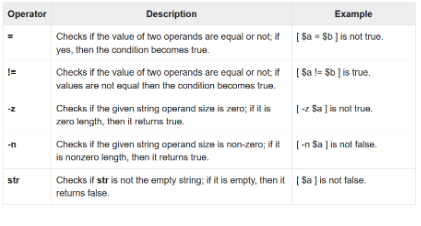
\includegraphics{string_operator.png}
}
\end{center}

\addcontentsline{toc}{section}{Unnumbered Section}
\section*{File Test Operators}
We have a few operators that can be used to test various properties associated with a Unix file.\\
Assume a variable file holds an existing file name "test" the size of which is 100 bytes and has read, write and execute permission on :\\
\begin{center}
    \resizebox{0.7\textwidth}{!}{
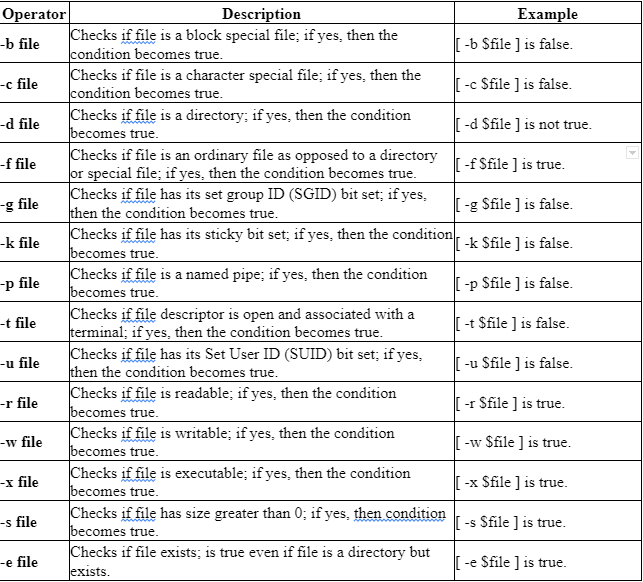
\includegraphics{file_operator.png}
}
\end{center}
Now we will understand shell decision-making in Unix. While writing a shell script, there may be a situation when you need to adopt one path out of the given two paths. So you need to make use of conditional statements that allow your program to make correct decisions and perform the right actions.\\
Unix Shell supports conditional statements which are used to perform different actions based on different conditions. We will now understand two decision-making statements here :\\
    The if...else statement\\
    The case...esac statement\\
The if...else statements\\
If else statements are useful decision-making statements which can be used to select an option from a given set of options.\\
Unix Shell supports following forms of if…else statement :\\
    if...if statement\\
    if...else...if statement\\
    if...elif...else...if statement\\
Most of the if statements check relations using relational operators discussed in the previous chapter.\\
The case...esac Statement\\
You can use multiple if...elif statements to perform a multiway branch. However, this is not always the best solution, especially when all of the branches depend on the value of a single variable.\\
Unix Shell supports case...esac statement which handles exactly this situation, and it does so more efficiently than repeated if...elif statements.\\
There is only one form of case...esac statement which has been described in detail here :\\
    case...esac statement\\
The case...esac statement in the Unix shell is very similar to the switch...case statement we have in other programming languages like C or C++ and PERL, etc.\\
In this chapter, we will discuss shell loops in Unix. A loop is a powerful programming tool that enables you to execute a set of commands repeatedly. In this chapter, we will examine the following types of loops available to shell programmers :\\
    The while loop\\
    The for loop\\
    The until loop\\
    The select loop\\
You will use different loops based on the situation. For example, the while loop executes the given commands until the given condition remains true; the until loop executes until a given condition becomes true.\\
Once you have good programming practice you will gain the expertise and thereby, start using appropriate loop based on the situation. Here, while and for loops are available in most of the other programming languages like C, C++ and PERL, etc.

\addcontentsline{toc}{section}{Unnumbered Section}
\section*{Nesting Loops}
All the loops support nesting concept which means you can put one loop inside another similar one or different loops. This nesting can go up to unlimited number of times based on your requirement.\\
Here is an example of nesting while loop. The other loops can be nested based on the programming requirement in a similar way 

\addcontentsline{toc}{section}{Unnumbered Section}
\section*{Nesting while Loops}
It is possible to use a while loop as part of the body of another while loop.\\
Syntax:\\
while command1 ; \# this is loop1, the outer loop\\
do\\
   Statement(s) to be executed if command1 is true\\
   while command2 ; \# this is loop2, the inner loop\\
   do\\
      Statement(s) to be executed if command2 is true\\
   done\\
   Statement(s) to be executed if command1 is true\\
done\\
Example\\
Here is a simple example of loop nesting. Let's add another countdown loop inside the loop that you used to count to nine :\\
\#!/bin/sh\\
a=0\\
while [ "\$a" -lt 10 ]    \# this is loop1\\
do\\
   b="\$a"\\
   while [ "\$b" -ge 0 ]  \# this is loop2\\
   do\\
      echo -n "\$b "\\
      b=`expr \$b - 1`\\
   done\\
   echo\\
   a=`expr \$a + 1`\\
done\\
This will produce the following result. It is important to note how echo -n works here. Here -n option lets echo avoid printing a new line character.\\
0\\
1 0\\
2 1 0\\
3 2 1 0\\
4 3 2 1 0\\
5 4 3 2 1 0\\
6 5 4 3 2 1 0\\
7 6 5 4 3 2 1 0\\
8 7 6 5 4 3 2 1 0\\
9 8 7 6 5 4 3 2 1 0\\
In this chapter, we will discuss shell loop control in Unix. So far you have looked at creating loops and working with loops to accomplish different tasks. Sometimes you need to stop a loop or skip iterations of the loop.\\
Now we will learn following two statements that are used to control shell loops

\addcontentsline{toc}{section}{Unnumbered Section}
\section*{The break statements}
The infinite Loop\\
All the loops have a limited life and they come out once the condition is false or true depending on the loop.\\
A loop may continue forever if the required condition is not met. A loop that executes forever without terminating executes for an infinite number of times. For this reason, such loops are called infinite loops.\\
Example:\\
Here is a simple example that uses the while loop to display the numbers zero to nine :\\
\#!/bin/sh\\
a=10\\
until [ \$a -lt 10 ]\\
do\\
   echo \$a\\
   a=`expr \$a + 1`\\
done\\
This loop continues forever because a is always greater than or equal to 10 and it is never less than 10.\\
The break Statement\\
The break statement is used to terminate the execution of the entire loop, after completing the execution of all of the lines of code up to the break statement. It then steps down to the code following the end of the loop.\\
Syntax:\\
The following break statement is used to come out of a loop :\\
break\\
The break command can also be used to exit from a nested loop using this format :\\
break n\\
Here n specifies the nth enclosing loop to the exit from.\\
Example:\\
Here is a simple example which shows that loop terminates as soon as a becomes 5 :\\
\#!/bin/sh\\
a=0\\
while [ \$a -lt 10 ]\\
do\\
   echo \$a\\
   if [ \$a -eq 5 ]\\
   then\\
      break\\
   if
   a=`expr \$a + 1`\\
done\\
Upon execution, you will receive the following result :\\
0\\
1\\
2\\
3\\
4\\
5\\
Here is a simple example of nested for loop. This script breaks out of both loops if var1 equals 2 and var2 equals 0 ;\\
\#!/bin/sh\\
for var1 in 1 2 3\\
do\\
   for var2 in 0 5\\
   do\\
      if [ \$var1 -eq 2 -a \$var2 -eq 0 ]\\
      then\\
         break 2\\
      else\\
         echo "\$var1 \$var2"\\
      fi\\
   done\\
done\\
Upon execution, you will receive the following result. In the inner loop, you have a break command with the argument 2. This indicates that if a condition is met you should break out of outer loop and ultimately from the inner loop as well.\\
1 0\\
1 5\\

\addcontentsline{toc}{section}{Unnumbered Section}
\section*{The Continue statements}
The continue statement is similar to the break command, except that it causes the current iteration of the loop to exit, rather than the entire loop.\\
This statement is useful when an error has occurred but you want to try to execute the next iteration of the loop.\\
continue\\
Like with the break statement, an integer argument can be given to the continue command to skip commands from nested loops.\\
continue n\\
Here n specifies the nth enclosing loop to continue from.\\
Example\\
The following loop makes use of the continue statement which returns from the continue statement and starts processing the next statement :\\
\#!/bin/sh\\
NUMS="1 2 3 4 5 6 7"\\
for NUM in \$NUMS\\
do\\
   Q=`expr \$NUM \% 2`\\
   if [ \$Q -eq 0 ]\\
   then\\
      echo "Number is an even number!!"\\
      continue\\
   fi\\
   echo "Found odd number"\\
done\\
Upon execution, you will receive the following result :\\
Found odd number\\
Number is an even number!!\\
Found odd number\\
Number is an even number!!\\
Found odd number\\
Number is an even number!!\\
Found odd number\\

\addcontentsline{toc}{section}{Unnumbered Section}
\section*{Substitution}
The shell performs substitution when it encounters an expression that contains one or more special characters.\\
Example\\
Here, the printing value of the variable is substituted by its value. Same time, "\n" is substituted by a new line :\\
\#!/bin/sh\\
a=10\\
echo -e "Value of a is \$a \n"\\
You will receive the following result. Here the -e option enables the interpretation of backslash escapes.\\
Value of a is 10\\
Following is the result without -e option −\\
Value of a is 10\n\\
The following escape sequences which can be used in echo command −\\
\begin{center}
    \resizebox{0.7\textwidth}{!}{
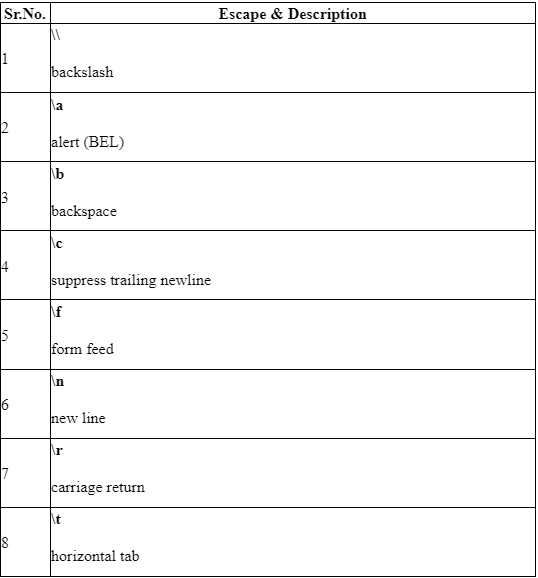
\includegraphics{substitution.png}
}
\end{center}
We can use the -E option to disable the interpretation of the backslash escapes (default).\\
We can use the -n option to disable the insertion of a new line.\\

\addcontentsline{toc}{section}{Unnumbered Section}
\section*{Command Substitution}
Command substitution is the mechanism by which the shell performs a given set of commands and then substitutes their output in the place of the commands.\\
Syntax:\\
The command substitution is performed when a command is given as :\\
`command`\\
When performing the command substitution make sure that you use the backquote, not the single quote character.\\\
Example:\\
Command substitution is generally used to assign the output of a command to a variable. Each of the following examples demonstrates the command substitution :\\
\#!/bin/sh\\
DATE=`date`\\
echo "Date is \$DATE"\\
USERS=`who | wc -l`\\
echo "Logged in user are \$USERS"\\
UP=`date ; uptime`\\
echo "Uptime is \$UP"\\
Upon execution, you will receive the following result :\\
Date is Thu Jul  2 03:59:57 MST 2021\\
Logged in user are 1\\
Uptime is Thu Jul  2 03:59:57 MST 2021\\
03:59:57 up 20 days, 14:03,  1 user,  load avg: 0.13, 0.07, 0.15\\

\addcontentsline{toc}{section}{Unnumbered Section}
\section*{Command Substitution}
Variable substitution enables the shell programmer to manipulate the value of a variable based on its state.\\
Here is the following table for all the possible substitutions :\\
\begin{center}
    \resizebox{0.7\textwidth}{!}{
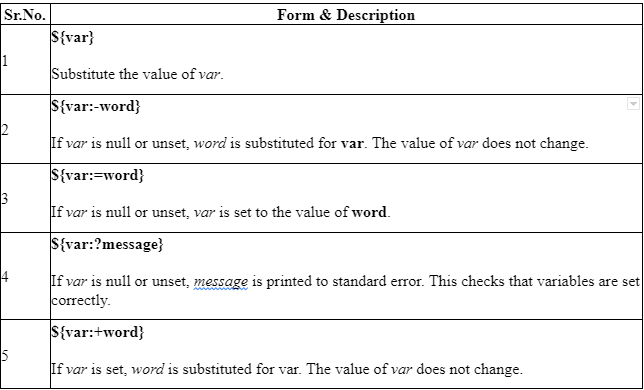
\includegraphics{variable_substitution.png}
}
\end{center}
Example:\\
Following is the example to show various states of the above substitution :\\
\#!/bin/sh\\
echo \${var:-"Variable is not set"}\\
echo "1 - Value of var is \${var}"\\
echo \${var:="Variable is not set"}\\
echo "2 - Value of var is \${var}"\\
unset var\\
echo \$\{var:+"This is default value"\}\\
echo "3 - Value of var is \$var"\\
var="Prefix"\\
echo \$\{var:+"This is default value"\}\\
echo "4 - Value of var is \$var"\\
echo \$\{var:?"Print this message"\}\\
echo "5 - Value of var is \$\{var\}"\\
Upon execution, you will receive the following result :\\
Variable is not set\\
1 : Value of var is\\
Variable is not set\\
2 : Value of var is Variable is not set\\
3 : Value of var is\\
This is default value\\
4 : Value of var is Prefix\\
Prefix\\
5 : Value of var is Prefix


\addcontentsline{toc}{section}{Unnumbered Section}
\section*{Shell Quoting Mechanisms}
The Metacharacters\\
Unix Shell provides various metacharacters which have special meaning while using them in any Shell Script and causes termination of a word unless quoted.\\
For example, ? matches with a single character while listing files in a directory and an * matches more than one character. Here is a list of most of the shell special characters (also called metacharacters) :\\
* ? [ ] ' " \ \$ ; & ( ) | \^ $<$ $>$ new-line space tab\\
A character may be quoted (i.e., made to stand for itself) by preceding it with a \$\$.\\
Example\\
Following example shows how to print a * or a ? −\\
\#!/bin/sh\\
echo Hello; Word\\
Upon execution, you will receive the following result :\\
Hello\\
./test.sh: line 2: Word: command not found\\
shell returned 127\\
Let us now try using a quoted character :\\
\#!/bin/sh\\
echo Hello\; Word\\
Upon execution, you will receive the following result :\\
Hello; Word\\
The \$ sign is one of the metacharacters, so it must be quoted to avoid special handling by the shell :\\
\#!/bin/sh\\
echo "I have \$1200"\\
Upon execution, you will receive the following result :\\
I have \$1200\\
The following table lists the four forms of quoting 
\begin{center}
    \resizebox{0.7\textwidth}{!}{
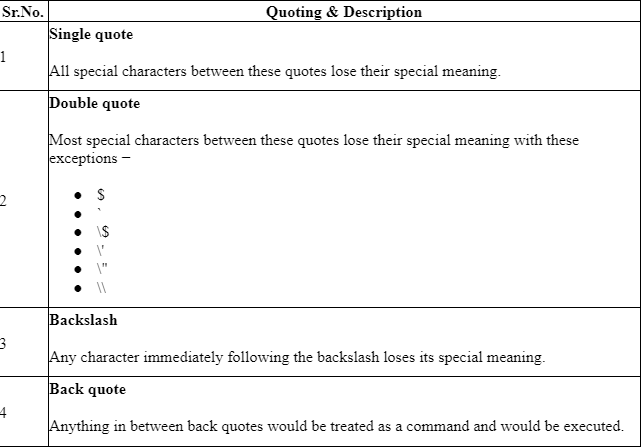
\includegraphics{quoating.png}
}
\end{center}

\addcontentsline{toc}{section}{Unnumbered Section}
\section*{The Single Quotes}
Consider an echo command that contains many special shell characters :\\
echo $<$-\$1500.**$>$; (update?) [y|n]\\
Putting a backslash in front of each special character is tedious and makes the line difficult to read :\\
echo \$<$-\$1500.\*\*\$>$\; \(update\?\) \[y\|n\]\\
There is an easy way to quote a large group of characters. Put a single quote (') at the beginning and at the end of the string :\\
echo '$<$-\$1500.**$>$; (update?) [y|n]'\\
Characters within single quotes are quoted just as if a backslash is in front of each character. With this, the echo command displays in a proper way.\\
If a single quote appears within a string to be output, you should not put the whole string within single quotes instead you should precede that using a backslash (\\) as follows :\\
echo 'It\'s Shell Programming\\
The Double Quotes\\
Try to execute the following shell script. This shell script makes use of single quote :\\
VAR=SIDDHARTHA\\
echo '\$VAR owes $<$-\$1500.**$>$; [ as of (`date +\%m/\%d`) ]'\\
Upon execution, you will receive the following result :\\
\$VAR owes $<$-\$1500.**$>$; [ as of (`date +\%m/\%d`) ]\\
This is not what had to be displayed. It is obvious that single quotes prevent variable substitution. If you want to substitute variable values and to make inverted commas work as expected, then you would need to put your commands in double quotes as follows :\\
VAR=SIDDHARTHA\\
echo "\$VAR owes <-\$1500.**$>$; [ as of (`date +\%m/\%d`) ]"\\
Upon execution, you will receive the following result −
SIDDHARTHA owes <-\$1500.**$>$; [ as of (07/02) ]\\
Double quotes take away the special meaning of all characters except the following :\\
    \ for parameter substitution\\
    Backquotes for command substitution\\
    \$ to enable literal dollar signs\\
    \` to enable literal backquotes\\
    \" to enable embedded double quotes\\
    $\\$ to enable embedded backslashes\\
    All other \ characters are literal (not special)\\
Characters within single quotes are quoted just as if a backslash is in front of each character. This helps the echo command display properly.\\
If a single quote appears within a string to be output, you should not put the whole string within single quotes instead you should precede that using a backslash (\\) as follows :\\
echo 'It\'s Shell Programming'\\
The Backquotes\\
Putting any Shell command in between backquotes executes the command.\\
Syntax\\
Here is the simple syntax to put any Shell command in between backquotes :\\
var=`command`\\
Example:\\
The date command is executed in the following example and the produced result is stored in DATA variable.\\
DATE=`date`\\
echo "Current Date: \$DATE"\\
Upon execution, you will receive the following result :\\
Current Date: Thu Jul  2 05:28:45 MST 2009\\

\addcontentsline{toc}{section}{Unnumbered Section}
\section*{Shell Input/Output Redirections}
Now we will discuss in detail about the Shell input/output redirections. Most Unix system commands take input from your terminal and send the resulting output back to your terminal. A command normally reads its input from the standard input, which happens to be your terminal by default. Similarly, a command normally writes its output to standard output, which is again your terminal by default.

\addcontentsline{toc}{section}{Unnumbered Section}
\section*{Output Redirection}
The output from a command normally intended for standard output can be easily diverted to a file instead. This capability is known as output redirection.
If the notation $>$ file is appended to any command that normally writes its output to standard output, the output of that command will be written to file instead of your terminal.\\
Check the following who command which redirects the complete output of the command in the users file.\\
\$ who $>$ users\\
Notice that no output appears at the terminal. This is because the output has been redirected from the default standard output device (the terminal) into the specified file. You can check the users file for the complete content :\\
\$ cat users\\
oko         tty01   Sep 12 07:30\\
ai          tty15   Sep 12 13:32\\
ruth        tty21   Sep 12 10:10\\
pat         tty24   Sep 12 13:07\\
steve       tty25   Sep 12 13:03\\
\$\\
If a command has its output redirected to a file and the file already contains some data, that data will be lost. Consider the following example :\\
\$ echo line 1 $>$ users\\
\$ cat users\\
line 1\\
\$\\
You can use $>$ $>$ operator to append the output in an existing file as follows :\\
\$ echo line 2 $>$ $>$ users\\
\$ cat users\\
line 1\\
line 2\\
\$\\
Input Redirection\\
Just as the output of a command can be redirected to a file, so can the input of a command be redirected from a file. As the greater-than character > is used for output redirection, the less-than character < is used to redirect the input of a command.\\
The commands that normally take their input from the standard input can have their input redirected from a file in this manner. For example, to count the number of lines in the file users generated above, you can execute the command as follows −
\$ wc -l users\\
2 users\\
\$\\
Upon execution, you will receive the following output. You can count the number of lines in the file by redirecting the standard input of the wc command from the file users :\\
\$ wc -l $<$ users\\
2\\
\$\\
Note that there is a difference in the output produced by the two forms of the wc command. In the first case, the name of the file users is listed with the line count; in the second case, it is not.\\
In the first case, wc knows that it is reading its input from the file users. In the second case, it only knows that it is reading its input from standard input so it does not display file name.\\

\addcontentsline{toc}{section}{Unnumbered Section}
\section*{Here Document}
A here document is used to redirect input into an interactive shell script or program.\\
We can run an interactive program within a shell script without user action by supplying the required input for the interactive program, or interactive shell script.\\
The general form for a here document is :\\
command $<$ $<$ delimiter\\
document\\
delimiter\\
Here the shell interprets the << operator as an instruction to read input until it finds a line containing the specified delimiter. All the input lines up to the line containing the delimiter are then fed into the standard input of the command.\\
The delimiter tells the shell that the here document has completed. Without it, the shell continues to read the input forever. The delimiter must be a single word that does not contain spaces or tabs.\\
Following is the input to the command wc -l to count the total number of lines −
\$wc -l $<$ $<$ EOF\\
   This is a simple lookup program \\
	for good (and bad) restaurants\\
	in Cape Town.\\
EOF\\
3\\
\$\\
You can use the here document to print multiple lines using your script as follows :\\
\#!/bin/sh\\
cat << EOF\\
This is a simple lookup program \\
for good (and bad) restaurants\\
in Cape Town.\\
EOF	\\
Upon execution, you will receive the following result :\\
This is a simple lookup program\\
for good (and bad) restaurants\\
in Cape Town.\\
The following script runs a session with the vi text editor and saves the input in the file test.txt.\\
\#!/bin/sh\\
filename=test.txt\\
vi \$filename $<$ $<$EndOfCommands\\
i\\
This file was created automatically from a shell script\\
\^[\\
ZZ\\
EndOfCommands\\
If you run this script with vim acting as vi, then you will likely see output like the following :\\
\$ sh test.sh\\
Vim: Warning: Input is not from a terminal\\
\$\\
After running the script, you should see the following added to the file test.txt :\\
\$ cat test.txt\\
This file was created automatically from a shell script\\
\$

\addcontentsline{toc}{section}{Unnumbered Section}
\section*{Discard the output}
Sometimes you will need to execute a command, but you don't want the output displayed on the screen. In such cases, you can discard the output by redirecting it to the file /dev/null :\\
\$ command $>$ /dev/null\\
Here command is the name of the command you want to execute. The file /dev/null is a special file that automatically discards all its input.\\
To discard both output of a command and its error output, use standard redirection to redirect STDERR to STDOUT :\\
\$ command $>$ /dev/null 2$>$\&1\\
Here 2 represents STDERR and 1 represents STDOUT. You can display a message on to STDERR by redirecting STDOUT into STDERR as follows :\\
\$ echo message 1$>$\&2\\

\addcontentsline{toc}{section}{Unnumbered Section}
\section*{Redirection Commands}
Following is a complete list of commands which you can use for redirection :
\begin{center}
    \resizebox{0.7\textwidth}{!}{
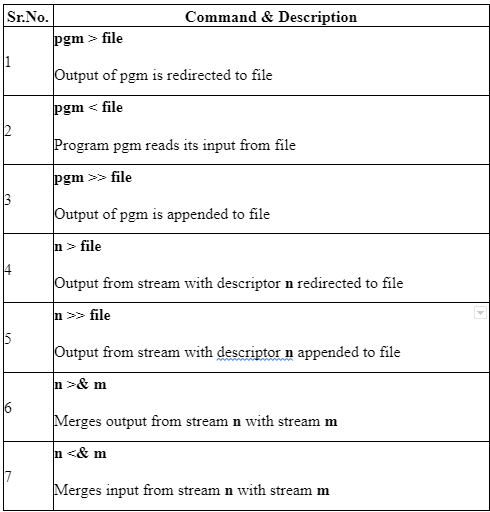
\includegraphics{redirection.png}
}
\end{center}

\addcontentsline{toc}{section}{Unnumbered Section}
\section*{Shell Functions}
Finally we will discuss in detail about the shell functions. Functions enable you to break down the overall functionality of a script into smaller, logical subsections, which can then be called upon to perform their individual tasks when needed.\\
Using functions to perform repetitive tasks is an excellent way to create code reuse. This is an important part of modern object-oriented programming principles.\\
Shell functions are similar to subroutines, procedures, and functions in other programming languages.\\

\addcontentsline{toc}{section}{Unnumbered Section}
\section*{Creating Functions}
To declare a function, simply use the following syntax :\\
function\_name () \{\\ 
   list of commands\\
\}\\
The name of your function is function\_name, and that's what you will use to call it from elsewhere in your scripts. The function name must be followed by parentheses, followed by a list of commands enclosed within braces.\\
Example:\\
Following example shows the use of function −\\
\#!/bin/sh\\
\# Define your function here\\
Hello () \{\\
   echo "Hello World"\\
\}\\
\# Invoke your function\\
Hello\\
Upon execution, you will receive the following output −\\
\$./test.sh\\
Hello World\\

\addcontentsline{toc}{section}{Unnumbered Section}
\section*{Pass Parameters to a Function}
You can define a function that will accept parameters while calling the function. These parameters would be represented by \$1, \$2 and so on.\\
Following is an example where we pass two parameters Zara and Ali and then we capture and print these parameters in the function.\\
\#!/bin/sh\\
\# Define your function here\\
Hello () \{\\
   echo "Hello World $1 $2"
\}\\
\# Invoke your function\\
Hello Siddhartha G\\
Upon execution, you will receive the following result :\\
\$./test.sh\\
Hello Siddhartha G\\

\addcontentsline{toc}{section}{Unnumbered Section}
\section*{Returning Values from Functions}
If you execute an exit command from inside a function, its effect is not only to terminate execution of the function but also of the shell program that called the function.\\
If you instead want to just terminate execution of the function, then there is way to come out of a defined function.\\
Based on the situation you can return any value from your function using the return command whose syntax is as follows \\

\addcontentsline{toc}{section}{Unnumbered Section}
\section*{return code}
Here code can be anything you choose here, but obviously you should choose something that is meaningful or useful in the context of your script as a whole.\\
Example\\
Following function returns a value 10 :\\
\#!/bin/sh\\
\# Define your function here\\
Hello () \{\\
   echo "Hello World $1 $2"
   return 10
\}\\
\# Invoke your function\\
Hello Siddhartha G\\
\# Capture value returned by last command\\
ret=\$?\\
echo "Return value is \$ret"\\
Upon execution, you will receive the following result :\\
\$./test.sh\\
Hello World Siddhartha G\\
Return value is 10\\
Nested Functions\\
One of the more interesting features of functions is that they can call themselves and also other functions. A function that calls itself is known as a recursive function.\\
Following example demonstrates nesting of two functions :\\
\#!/bin/sh\\
\# Calling one function from another\\
number\_one () \{\\
   echo "This is the first function speaking..."
   number\_two
\}\\
number\_two () \{\\
   echo "This is now the second function speaking..."
\}\\
\# Calling function one.\\
number\_one\\
Upon execution, you will receive the following result :\\
This is the first function speaking...\\
This is now the second function speaking...\\

\addcontentsline{toc}{section}{Unnumbered Section}
\section*{Function Call from Prompt}
You can put definitions for commonly used functions inside your .profile. These definitions will be available whenever you log in and you can use them at the command prompt.\\
Alternatively, you can group the definitions in a file, say test.sh, and then execute the file in the current shell by typing :\\
\$. test.sh\\
This has the effect of causing functions defined inside test.sh to be read and defined to the current shell as follows :\\
\$ number\_one\\
This is the first function speaking...\\
This is now the second function speaking...\\
\$\\
To remove the definition of a function from the shell, use the unset command with the .f option. This command is also used to remove the definition of a variable to the shell.\\
\$ unset -f function\_name\\
\end{document}